% !TEX root = ../thesis-example.tex
\chapter{Concepts}
\label{sec:concepts}

\section{Definitions}
\label{sec:concepts:defs}

In the following definitions are given to reason about semantics of implementations of a TeSSLa runtime.
A TeSSLa specification gives a number of transformations over input streams and a subset of the generated streams as outputs.
Streams can be queried for the value they hold at a specific time.

\subsection{Streams}
\label{sec:concepts:defs:streams}

There are two kind of streams: Signals, which carry values at all times and EventStreams, which only hold values at specific times.
EventStreams can be described by a sequence of Events, which hold a value and a timestamp: \((v_1,t_1),(v_2,t_2),\ldots\).
Signals can be described by a sequence of changes, which hold a value and a timestamp: \((v_1,t_1),(v_2,t_2),\ldots\).
This shows that the only difference between Signal and EventStreams is given, when we query the stream for it's value:
A Signal will always have a value, an EventStream may return \(\bot\), which denotes, that no event happened at that time.
Because the similarity of Signals and EventStreams in the following we will mainly reason about EventStreams, but most things can also be applied to Signals.

Futhermore Signals and EventStreams hold the timestamp to which they have progressed, which can be equal or greater than the timestamp of the last Event happened on them.

\subsection{Events}
\label{sec:concepts:defs:events}

Streams consists of Events (or changes, which can be modeled the same as events).
There are three Types of Events: Input, Output and Internal events.

Let \(E\) be the Set of valid input events (E for external) and \(e \in E\), where each event carries a value, which can be \emph{nothing}, a timestamp and the
stream it's perceived on (e.g.\ a function call of a specific function).
Further let \(O\) be the Set of valid output events and \(o \in O\), which have the same properties than input events, while their channel is specified by the TeSSLa specification.

Internal events are mostly an implementation detail, which denotes steps of computation inside the runtime:
Let the Set of valid internal events be \(N\).
Internal events also carry a value and a timestamp, but their stream is implicitly given by the node that produces the event.

\subsection{Functions}
\label{sec:concepts:defs:functions}

A TeSSLa specification consists of functions which manipulates streams and generate new streams.
TeSSLa itself defines a syntax to write a specification, a set of types and a standard library of functions, but an implementation is free to choose the functions it supports.
An example function is \(add(S_D,S_D) \rightarrow S_D\): It takes two Signals, which have to hold values of some numerical type, and produces a signal which holds values of the same type.
The produced stream can either be assigned to a named identifier (think: a variable) or directly be given to another function (function composition).

\subsection{Nodes}
\label{sec:concepts:defs:nodes}

Nodes are the atomic unit of computation for the evaluation of a TeSSLa specification.
A Node implements a single Function, e.g.:\ there is an \emph{AddNode} which takes two input Signals and produces a new Signal.
Therefore a Node is the concrete implementation of a function in a runtime for TeSSLa specifications.

Because Functions in TeSSLa specifications itself depend on other Functions, and these dependencies have to be circle free,
the specification can be represented as a DAG and the Nodes are also organized as a DAG\@.
Each Node has a State that can hold arbitrary data used for computation.
One part of the State is the History of a Node, which holds all Events received from it's predecessors, called it's inputs, and all produced Events of the Node, called it's output.

Nodes use a FIFO queue, provided by the Erlang plattform, to process new received Events in multiple steps:
\begin{enumerate}
  \item Add the new Event to the inputs
  \item Check if a new output Events can be produced (see Section~\ref{sec:concepts:defs:nodes:processable})
  \item If so, compute all timestamps, where new Events might be computed and
    \begin{enumerate}
      \item Compute the Events, add them to the History as new outputs
      \item Distribute the updated output to all successors
    \end{enumerate}
  \item Else wait for another input
\end{enumerate}

\subsubsection{Determination of processable Events}
\label{sec:concepts:defs:nodes:processable}

Based on the asynchronous nature of Nodes, Events from different channels can be received out of order.
E.g.\ if a Node C is a child of Node A and B, it can receive Events from Node A at timestamps \(t_1, t_2, t_3, t_4\)
before receiving an event with timestamp \(t_1\) from Node B.
Therefore a Node can not compute it's output upto a timestamp unless it has informations from all predecessors that they did progress to that timestamp.
When Node C receives the first four Events from Node A, it will only add them to it's inputs but won't compute an output.
When it finally receives the first Event from Node B it can compute all Events upto \(t_1\).
To do so it will compute \emph{change timestamps}: The union of all timestamps where an Event occured on any input between the timestamp of the last generated output and the minimal progress of all inputs.
To see why this is necessary lets assume that Node C will receive a new Event from Node B with timestamp \(t_4\):
All inputs have progressed to \(t_4\), but on the stream from Node A there are changes between \(t_1\) (where the last output was generated) and \(t_4\),
therefore the \emph{change timestamps} are \(t_2, t_3, t_4\) and the Node will have to compute it's output based on the values of the streams at that timestamps.

\subsection{TeSSLa Evaluation Model}
\label{sec:concepts:def:model}

Based on the format of TeSSLa specifications a specific structure for evaluation is given:
A DAG that consists of Nodes, where the roots are the ones consuming external Events and the leaves are the ones producing outputs.
The Nodes in the DAG are called \emph{ready} when they have at least one input buffered for all of their predecessors, meaning they are able to perform a computation and produce a new output.
In later sections the equality of different schedules of Nodes are shown.

\subsection{State}
\label{sec:concepts:def:state}

All TeSSLa runtimes have to have a State, which encodes information necessary to compute further Events.
The State of a whole Evaluation Engine is made up of the States of it's Nodes.
The State of a Node is made up of arbitrary Information needed to perform later computations, the events it generated and the queue of new inputs.

\subsection{Transitions}
\label{sec:concepts:def:transitions}

Transitions describe the Steps between two States an evaluation Engine takes: The consumption of an Event from all inputs of a Node and the production and propagation of a new output from that Node.

\subsection{Run}
\label{sec:concepts:def:run}

A Run of an Evaluation Engine is a Series of States and Transitions.
It is a representation of the steps the Engine takes to evaluate a specification over streams.
The run \(s_0\theta_1s_1\) means, that the Engine was in it's initial State, took the transition \(\theta_1\) and thereby reached the state \(s_1\).

% TODO


% \cleanchapterquote{Innovation distinguishes between a leader and a follower.}{Steve Jobs}{(CEO Apple Inc.)}
% \section{Semantics of TeSSLa functions}
% \label{sec:concepts:semantics_tessla_functions}
% Think of semantics of thinks like add, mrv, etc.
% Can these be defined independent of async/synchronous or for each.
% For synchronous they are partly defined in the TeSSLa spec

\section{Behaviour of different evaluation strategies without timing functions}
\label{sec:concepts:behaviour_without_timing}

For a first step we specify and compare behaviours of different approaches to evaluate TeSSLa specifications without timing formulas,
meaning that only functions, which manipulate values or the presence of events, but not the timestamp of them, are used.
This leads to behaviours that can be easily reason about, as seen in the next sections.

All Evaluation Engines compute Events in steps.
Each step a Node is scheduled to perform it's specific Task, therefore one of the following things can happen in each step.

\begin{itemize}
  \item An input Event can be consumed by a source in the DAG, which generates an internal event that is propagated to it's children
  \item An internal Node which has at least one new input buffered on all of its input queues can perform
    it's computation and generate a new internal event, which is propagated to the children of that node, which therefore can compute in the next step.
  \item An output node, which has at least one new input buffered on its input queue, can produce a new output.
\end{itemize}

The difference between Evaluation Engines is the way they are scheduling the Nodes.
In the following we will define different ways of scheduling and proove equality between them.

\subsection{Synchronous evaluation}
\label{sec:concepts:behaviour_without_timing:synchronous}

An synchronous System \(I\) for a specification \(T\) is one that has a fixed schedule build like this:
Number all Nodes in a reversed topological order once, then always schedule the ready Node with the lowest number.
Obiously for many DAGs there is no unique reversed topological order, therefore one has to be chosen.
This schedule ensures that no new events are consumed by any predecessor of a Node that is ready itself, therefore Events are \emph{pushed} through the DAG towards an output Node as fast as possible.

The synchronous system can be considered as the \emph{Source of Truth}: The Relationship between inputs and outputs it generates
is assumed to be the right evaluation for a given TeSSLa specification.
All other approaches must generate a relationship between inputs and outputs that can be transformed into the one from the synchronous system,
or else the different approach is not seen as a valid system for the specification.

Figure~\ref{fig:chap3:sec_sync:visual_dag} visualizes a synchronous System.
It shows two DAG representations of an evaluation Engine  where the Nodes A to E are labeled in a reversed topological order and \(o_1\) and \(o_2\) represents the output channels with that name.
The left System is in it's initial State and an input event \(\langle e_1,t_1\rangle\) is ready to be consumed.
When a Node is chosen to compute by the scheduler, only Node A is ready, therefore it is scheduled.
The right system is the representation of the next step: Node A has consumed the external event and produced an internal event \(\langle n_A,t_1\rangle\) which is propagated to all it's children: Node B and D.
In the next step Node B would be scheduled, because it has the lowest number of any node that can compute (actually it's the only node that can compute at all, because D has to wait for the event from B).
After B was scheduled, it would have produced the internal Event \(\langle n_B,t_1\rangle\) which would then be distributed to Nodes C and D.
Therefore the trace of consumed external and produced internal and output events by the system with this specific schedule could be visualized as: % TODO replace with run
\[
  \langle e_1,t_1 \rangle \langle n_{A1},t_1 \rangle \langle n_{B1},t_1 \rangle \langle n_{C1},t_1 \rangle \langle o_{1,1},t_1 \rangle \langle n_{D1},t_1 \rangle \langle n_{E1},t_1 \rangle \langle o_{2,1},t_1 \rangle
\]
If there were more than one input event, at this point Node A would be scheduled again, consume the next external event and the following nodes would be scheduled in the same order as before,
extending the trace in an obvious way.

\begin{figure}
  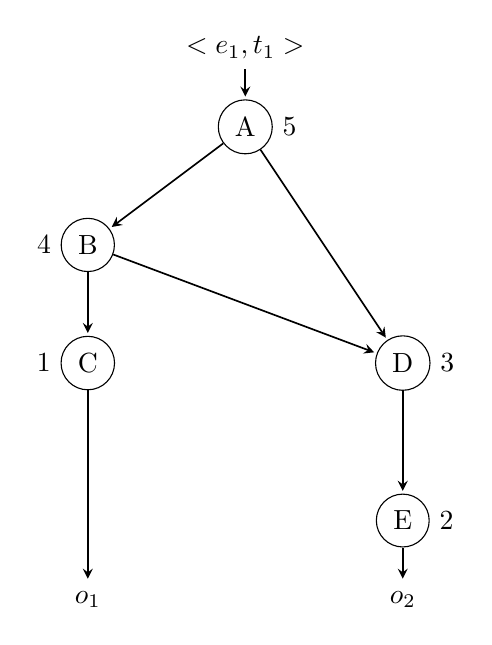
\begin{tikzpicture}
    [pre/.style={<-,shorten <=1pt,>=stealth,semithick}]
    \node (S) at (2,5) {\(<e_1,t_1>\)};
    \node [shape=circle,draw=black] (A) [label=right:5] at (2, 4) {A}
      edge [pre] (S);
    \node [shape=circle,draw=black] (B) [label=left:4] at (0,2.5) {B}
      edge [pre] (A);
    \node [shape=circle,draw=black] (C) [label=left:1] at (0,1) {C}
      edge [pre] (B);
    \node [shape=circle,draw=black] (D) [label=right:3] at (4,1) {D}
      edge [pre] (A)
      edge [pre] (B);
    \node [shape=circle,draw=black] (E) [label=right:2] at (4,-1) {E}
      edge [pre] (D);
    \node (o1) at (0,-2) {\(o_1\)} edge [pre] (C);
    \node (o2) at (4,-2) {\(o_2\)} edge [pre] (E);
  \end{tikzpicture}
  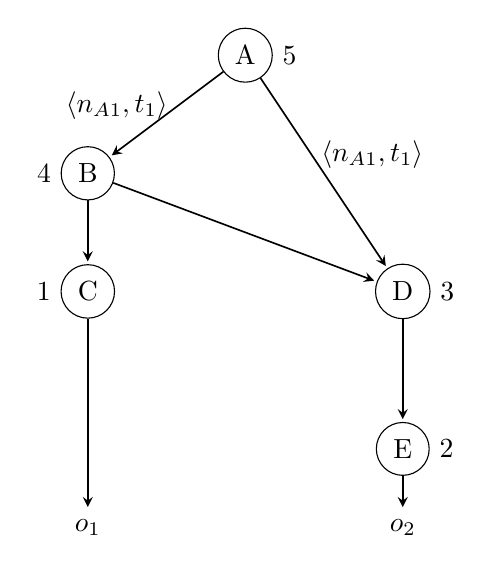
\begin{tikzpicture}
    [pre/.style={<-,shorten <=1pt,>=stealth,semithick}]
    \node [shape=circle,draw=black] (A) [label=right:5] at (2, 4) {A};
    \node [shape=circle,draw=black] (B) [label=left:4] at (0,2.5) {B}
      edge [pre] node[align=left,left,pos=0.6] {\(\langle n_{A1},t_1\rangle\)} (A);
    \node [shape=circle,draw=black] (C) [label=left:1] at (0,1) {C}
      edge [pre] (B);
    \node [shape=circle,draw=black] (D) [label=right:3] at (4,1) {D}
      edge [pre] node[align=right,right,pos=0.6] {\(\langle n_{A1},t_1\rangle\)} (A)
      edge [pre] (B);
    \node [shape=circle,draw=black] (E) [label=right:2] at (4,-1) {E}
      edge [pre] (D);
    \node (o1) at (0,-2) {\(o_1\)} edge [pre] (C);
    \node (o2) at (4,-2) {\(o_2\)} edge [pre] (E);
  \end{tikzpicture}
  \caption{Visualization of a simple asynchronous system with a reversed topological order.}
\label{fig:chap3:sec_sync:visual_dag}
\end{figure}
% The behaviour for a single input can be described by two functions:

% \begin{align*}
%   \Phi&: S \times E \rightarrow S \\
%   \Theta&: S \times E \rightarrow O^*
% \end{align*}

% The behaviour for multiple inputs is the composition of the functions.

% The trace for the implementation \(I\) for a Stream of input events from \(E^*\) is given by the output Stream
% from \(O^*\) that is generated by the formulas.

% The processing of a series of 3 input events of a synchronous system can be visualized like shown in Figure~\ref{fig:chap3:sec_sync:form_sync_processing}.

% \begin{figure}
%   \begin{flalign*}
%     &\text{Timestamp:}  && t_0      &&t_1\                          &&t_2                        &&t_3 &\\
%     &\text{Input:}      &&          &&e_1\                          &&e_2                        &&e_3 &\\
%     &\text{State:}      && I_0      &&I_1\                          &&I_2                        &&I_3 &\\
%     &\text{Outputs:}    &&          &&(o_{1,1}, \dots, o_{1,x})     &&(o_{2,1}, \dots, o_{2,y})  &&(o_{3,1}, \dots, o_{3,z}) &
%   \end{flalign*}
%   \caption{Example computation of 3 Inputs by an synchronous implementation}
% \label{fig:chap3:sec_sync:form_sync_processing}
% \end{figure}

\subsection{Asynchronous evaluation}
\label{sec:concepts:behaviour_without_timing:async}

An asynchronous system \(A\) for a specification \(T\) is a Evaluation Engine with a fair, but not fixed schedule.

% The asynchronous system doesn't consider a number of implementation details of the actual implementation, e\.g\. the needed computation duration of a Node:
% Each Node takes exactly one step to produce a new output based on inputs.

% The asynchronous system has a more complex behaviour than the synchronous system because Nodes have to wait for other Nodes that are before them
% and there are multiple Nodes that can produce outputs.

% It's state is defined by the product of the States of it's nodes, where each node represents a primitive operation in
% the specification and the nodes are organized as a DAG.%TODO glossary
% The output is specified by the concatination of outputs of the nodes that are marked as output nodes in the specification.



% TODO Proove equality between different topological orders
% TODO also sth\. about multiple nodes computing at once == (one node at a time + fairness)
In contrast to the synchronous evaluation Engine it has no fixed schedule, the only requirement is that the schedule is fair.
Therefore predecessors of ready Nodes can perform multiple computations before their children are scheduled and Events are not \emph{pushed} thorugh the DAG as fast as possible.

\section{Equalitys of different Systems without timing functions}
\label{sec:concepts:equalitys_without_timing}

Based on the described behaviours of the approaches we now can proof the equality of them.

As already stated in Section~\ref{sec:concepts:behaviour_without_timing:synchronous} a synchronous evaluation engine is regarded as the source of truth, therefore all other kinds of evaluation engine have to be equal to one.

The equality is shown in two steps: First in Section~\ref{sec:concepts:equalitys_without_timing:synchronous}it is shown, that all possible synchronous Systems for a specification are equal, so there is only one true evaluation.
Afterwards in Section~\ref{sec:concepts:equalitys_without_timing:sync_async} it is shown that any asynchronous evaluation engine is equal to a synchronous one.
\subsection{Equality of synchronous Systems}
\label{sec:concepts:equalitys_without_timing:synchronous}

When given a series of input events, two synchronous evaluation Engines with different schedules will generate different runs,
but both will produce all outputs that can be produced after consuming one specific input
before the next Input is consumed as reasoned in Section~\ref{sec:concepts:behaviour_without_timing:synchronous}.

To proof the equality of both systems we have to proof the equality of their runs.
To do this we will show that any two runs of two synchronous system can be iteratively reordered without violation of causality until they are equal.

Let \(\vec{e} = (e_1, e_2, \dots, e_x)\) be the input events both implementations receive.
Furthermore let \(R_1, R_2\) be the runs of the two Systems for a given TeSSLa specification.

Because each TeSSLa specification contains only a finite amount of functions and works on finite traces, the runs also have to be finite.
When two Systems have a different schedule, their Runs will be different at a finite number of positions.
Let \(R'\) be the finite prefix of both runs that are equal (This will be at least \(s_0\), but possible more) and \(i_d\) the index of the first difference.
This means that at Step \(i\) the second evaluation engine has taken a different transition, meaning a different Node was scheduled at that point, than the first evaluation engine.

Let \(N_1\) be the Node scheduled by the first evaluation Engine and \(N_2\) by the second.
Because \(N_1\) was scheduled by the first evaluation engine, it also has to be ready in the second engine, and because it wasn't scheduled by it, it has to still be ready after that step.
The same holds for \(N_2\) in the first evaluation engine.
After step \(i_d\) both system might take a finite number of different transitions, but at some point the first System has to schedule Node \(N_2\) and the second system Node \(N_1\), because there are only a finite number of Nodes with a lower number and a Node can only become \emph{not ready} by performing it's computation.
Let \(i_{N_2} > i_d\) be the index of the step where the first System schedules the Node \(N_2\).
Let \(N_b\) be the set of all Nodes which were scheduled between \(i_d\) and \(i_{N_2}\).
None of theese Nodes can be a children of \(N_2\), because otherwise that Node couldn't be scheduled before \(N_2\), because it would have had to wait for an Event from \(N_2\).
Now let \(N_c \in N_b\) be the Node that was scheduled at step \(i_{N_2} - 1\) and
\(r_s = (\langle \tau_{i_{N_2} - 2}, s_{i_{N_2} - 2}\rangle, \langle\tau_{i_{N_2} - 1}, s_{i_{N_2} - 1}\rangle \langle\tau_{i_{N_2}}, s_{i_{N_2}}\rangle)\)
the suffix of the run from the first system from two steps before \(N_2\) was scheduled upto the point where it was scheduled.

Figure~\ref{fig:chap3:sec_sync:commutativity_scheduling} shows how changing the order of the Nodes \(N_c,N_2\) has no influence on the state after both have executed.
This is, because none of the two Nodes can be a children of the other, therefore only the state of other Nodes can change when one of them computes (by adding their generated events to their input queue).
If both Nodes have the same child, it will receive the inputs in different order, but because they're happening on different channels it doesn't matter.


\begin{figure}
  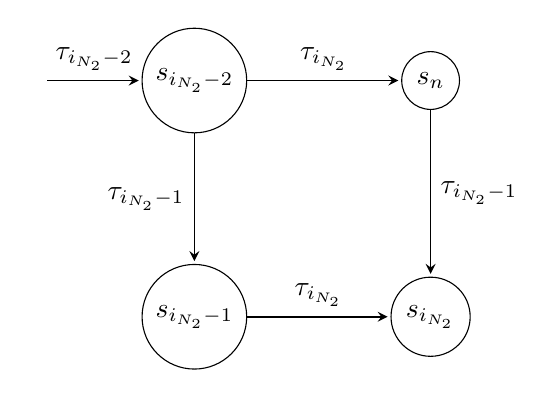
\begin{tikzpicture}
    [pre/.style={<-,shorten <=1pt,>=stealth,semithick}]
    \node (A) at (0,0) {};
    \node [shape=circle,draw=black] (B) at (2, 0) {\(s_{i_{N_2}-2}\)}
      edge [pre] node[above] {\(\tau_{i_{N_2}-2}\)} (A);
    \node [shape=circle,draw=black] (C) at (2, -3) {\(s_{i_{N_2}-1}\)}
      edge [pre] node[left] {\(\tau_{i_{N_2}-1}\)} (B);
    \node [shape=circle,draw=black] (D) at (5, 0) {\(s_{n}\)}
      edge [pre] node[above] {\(\tau_{i_{N_2}}\)} (B);
    \node [shape=circle,draw=black] (E) at (5, -3) {\(s_{i_{N_2}}\)}
      edge [pre] node[right] {\(\tau_{i_{N_2}-1}\)} (D)
      edge [pre] node[above] {\(\tau_{i_{N_2}}\)} (C);
  \end{tikzpicture}
  \caption{Commutativity Diagramm of Node scheduling}
\label{fig:chap3:sec_sync:commutativity_scheduling}
\end{figure}


% Let's first reason about the easy case, were only one external event is received:
% In this case \(I\) has only two states, \(I_0,\ I_1\) and will only produces outputs once: \(o_{1,1}, \dots, o_{1,x}\).
% \(A\) will walk through multiple states, bound by the number of functions in the specification it's implementing.
% Because the specification is a DAG, especially has no circles, eventually \(A\) has to finish it's computation, let the
% number of steps be \(k\).
% Let \(h_{\min}\) be the minimal height of the DAG (the height of the leave with the fewest steps to the Source).
% The first output can only be created after \(h_{\min}\) steps and after step \(k\) all outputs have to be created, so that
% \(o_{1,1}, \dots, o_{1,x}\) were emitted.
% Let the States of \(A\) during the computation be \(A_{0}, A_{1,0}, A_{1,1}, \dots, A_{1,k}\) where \(A_0\) is the initial state.

% When taking the first step and \(A_{1,0}\) is reached, the event \(e_1\) is consumed by a source node \(N_A\), which produces
% the internal event \(\langle n_{A,1},t_1\rangle\) and distributes it to it's children.
% Note that there is no alternative to this bahivour, because there were no prior events and therefore no internal Node
% has an event to process on it's input queue, therefore the Source consuming the external event is the only node that can,
% and therefore must, compute anything.
% Afterwards all Nodes that are direct children of the source that consumed the external event will have one input event buffered and
% are able to perform their computation in the next step.

% At least until step \(h_{\min}\) every step one or more Nodes, that are no outputs, will perform a computation, therefore
% pushing internal events closer to the output nodes.
% Somewhere between step \(h_{\min}\) and \(k\) all internal events will reach an output node and produce an output.

% A more complex case is when multiple external events are received.

% Because the scheduling of nodes of \(A\) is based on the reversed topological order, \(A\) will only consume one new external event and then will schedule internal nodes until all
% internal events have reached an output node, only than the next input will be consumed by a source node.
% \(I\) will step through a series of States \(I_0, I_1, \dots, I_x\), A on the other hand will step through a Series of
% states for each state that \(I\) takes: \(A_0,A_{1,0},A_{1,1},\dots,A_{1,j1},A_{2,0}, \dots,A_{x,j2}\) and generate internal events along those steps.
% Based on this behaviour lets define when a State of \(A\) is equal to one of \(I\):
% The first states \(A_0\) and \(I_0\) are always assumed to be equal, because no output can be observed and therefore one
% can't observe a difference.
% A State \(A_{i,j}\) with \(j > 0\) is called equal to a State \(I_{i}\) iff:

% \begin{itemize}
%   \item The previous state \(A_{i,j-1}\) was equal to \(I_{i}\)
%   \item and either
%     \begin{itemize}
%       \item No new output was generated at state \(A_{i,j}\)
%       \item or if a new output \(o\) is created it is equal to one of the outputs of \(I_{i}\) that wasn't generated before
%     \end{itemize}
% \end{itemize}

% A State \(A_{i,0}\) is called equal to a state \(I_{i}\) iff

% \begin{itemize}
%   \item The previous state \(A_{i-1,x}\) was equal to \(I_{i-1}\)
%   \item the input \(e_i\) was consumed at the step
%   \item and the States \(A_{i-1,0}\) to \(A{i-1,x}\) together produced the same output like \(I_{i-1}\)
% \end{itemize}

% Naively speaking the System \(A\) moves through states \(A_{i,0},\dots,A_{i,x}\) while it produces the same outputs as \(I\)
% produced when it reached state \(I_i\), and as soon as the last output was produced consumes a new event and thereby takes
% state \(A_{i+1,0}\).

% Based on this, a series of states \(\vec{A}\) is called equal to a series of States \(\vec{I}\) if each state in \(\vec{A}\)
% is equal to a state in \(\vec{I}\).
% The System \(A\) is equal to the system \(I\) in regard to a series of inputs \(\vec{e}\) iff all possible series of
% states it could take to process \(\vec{e}\) are equal to \(\vec{I}\).

\subsection{Equality of synchronous and asynchronous Systems}
\label{sec:concepts:equalitys_without_timing:sync_async}

When the Nodes of \(A\) aren't scheduled in reversed topological order, the system can consume Inputs before producing all outputs
based on the last consumed input.
Therefore the reordering of outputs and inputs (and internal events) has to be performed over the whole trace, not only between Input events.
Idea: each step is a commutation of two internal events in regard to the rev top order.
=> show commutativity of traces (note: only valid commutations, no two events, where one depends one the other, can be commuted, this is ensured by the scheduling of nodes that have input buffered)
